\chapter{Support Vector Machine}

\begin{multicols}{2}
\noindent SVMs are based on statistical learning theory. Basic idea behind SVMs is maximum margin
hyperplane.

\begin{center}
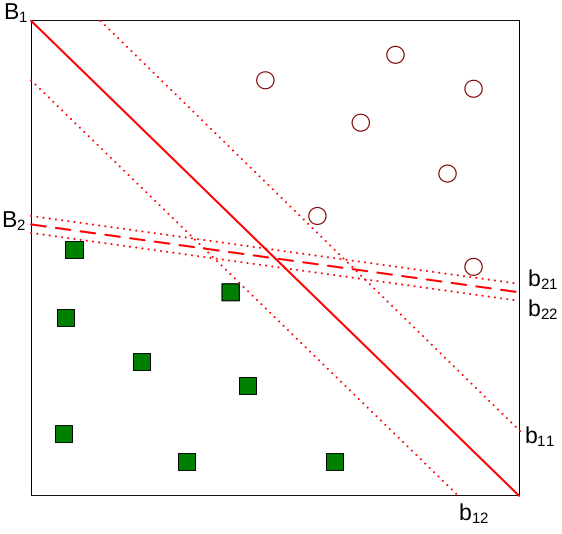
\includegraphics[width=5cm, height=5cm]{svm_margin}
\end{center}

\noindent Although all the hyperplanes shown in the figure can separate training examples perfectly, their generalization errors may be different. \\

\noindent Each decision boundary $B_i$ is associated with a pair of parallel hyperplanes $b_{i1}$ and $b_{i2}$. We assume that larger margins imply better generalization errors.

\section{Background: Inner Product}

\noindent The inner product of two vectors $\mathbf{u}$ and $\mathbf{v}$ is defined as:
$$\mathbf{u} \cdot \mathbf{v} = \|\mathbf{u} \|_2 \times \|\mathbf{v} \|_2 \times cos(\theta)$$
$$\|\mathbf{u} \|_2^2 = \mathbf{u} \cdot \mathbf{u} = \sum_{i=1}^d u_i \times u_i$$

\noindent As a result, $\mathbf{u}$ and $\mathbf{v}$ are orthogonal when $\theta$ is equal to $90\degree$

\begin{center}
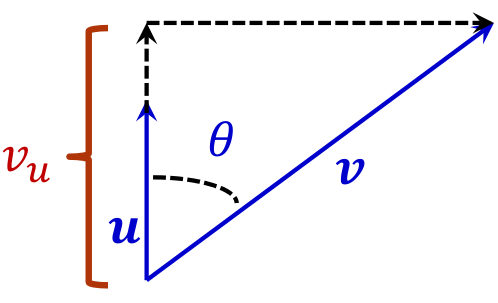
\includegraphics[width=5cm, height=3cm]{inner_projection}
\end{center}

\noindent Length of projection of vector $\mathbf{v}$ to $\mathbf{u}$:
\begin{equation*}
\begin{split}
    \mathbf{u} \cdot \mathbf{v} &= \|\mathbf{u} \|_2 \times \|\mathbf{v} \|_2 \times cos(\theta) \\
    &= \|\mathbf{u} \|_2 \times v_u
\end{split}
\end{equation*}

\section{Linear SVM}

\noindent Given a binary classification task, we define $y_i=+1$ as the circle class and $y_i=-1$ as the square class. The decision boundary of SVM is defined as:

$$\mathbf{w} \cdot \mathbf{x} + b = 0$$

\noindent For any test example $\mathbf{x^*}$:

$$
f(\mathbf{x^*}) = 
\begin{cases}
1 & \mathbf{w} \cdot \mathbf{x^*} + b \ge 0 \\
-1 & \mathbf{w} \cdot \mathbf{x^*} + b < 0
\end{cases}
$$

\subsection{Orthogonal of Weight}

\noindent The direction of $\mathbf{w}$ is orthogonal to the decision boundary. Suppose $\mathbf{x}_a$ and $\mathbf{x}_b$ are two points located on the decision boundary, then:
$$\mathbf{w} \cdot \mathbf{x}_a + b = 0$$
$$\mathbf{w} \cdot \mathbf{x}_b + b = 0$$
$$\mathbf{w} \cdot (\mathbf{x}_a -\mathbf{x}_b) = 0$$

\noindent Since $\mathbf{x}_a -\mathbf{x}_b$ represents a vector on the decision boundary and the inner product is equal to zero, so the direction of $\mathbf{w}$ is orthogonal to the decision boundary

\subsection{Equation of Parallel Hyperplane}

\noindent For any circle $\mathbf{x}_c$ located above the decision boundary:
$$\mathbf{w} \cdot \mathbf{x}_c + b = k, k>0$$
\noindent Similary, for any square $\mathbf{x}_s$ located below the decision boundary:
$$\mathbf{w} \cdot \mathbf{x}_s + b = k', k<0$$

\noindent The two parallel hyperplanes passing the closest circle and square can be written as:
$$\mathbf{w} \cdot \mathbf{x} + b = \bar{k}$$
$$\mathbf{w} \cdot \mathbf{x} + b = -\bar{k}$$

\noindent After rescaling $\mathbf{w}$ and $b$, the two parallel hyperplanes can be further rewritten as:
$$\mathbf{w} \cdot \mathbf{x} + b = 1$$
$$\mathbf{w} \cdot \mathbf{x} + b = -1$$

\subsection{Margin of SVM}
\begin{center}
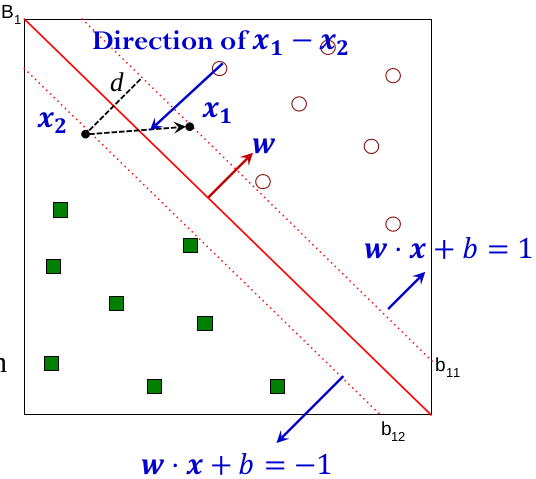
\includegraphics[width=5cm, height=5cm]{svm_margin_equation}
\end{center}
\noindent Let $\mathbf{x}_1$ and $\mathbf{x}_2$ be two points on two parallel hyperplanes:
$$\mathbf{w} \cdot \mathbf{x}_1 + b = 1$$
$$\mathbf{w} \cdot \mathbf{x}_2 + b = -1$$
$$\mathbf{w} \cdot (\mathbf{x}_1 - \mathbf{x}_2)= 2$$
\noindent Based on definition of inner product:
$$\| \mathbf{w} \|_2 \times d = 2$$
$$d = \frac{2}{\| \mathbf{w} \|_2}$$

\subsection{Learning in SVM}

\noindent We want to:
$$\!\min_w \frac{2}{\| \mathbf{w} \|_2^2}$$
$$\!\max_w \frac{\| \mathbf{w} \|_2^2}{2}$$

\noindent Subjected to the following constraints:
$$\mathbf{w} \cdot \mathbf{x}_i + b \ge 1, \text{if}\ y_i=1$$
$$\mathbf{w} \cdot \mathbf{x}_i + b \le 1, \text{if}\ y_i=-1$$

\noindent The constraints are equivalent to:
$$y_i \times (\mathbf{w} \cdot \mathbf{x}_i + b) \ge 1$$

\section{Linear SVM for Non-separable Classes}

\noindent We need to introduce slack variables $\xi \ge 0$ to absorb errors. \\

\noindent The constraints:
$$\mathbf{w} \cdot \mathbf{x}_i + b \ge 1 - \xi_i, \text{if}\ y_i=1$$
$$\mathbf{w} \cdot \mathbf{x}_i + b \le 1 - \xi_i, \text{if}\ y_i=-1$$

\noindent The constraints are equivalent to:
$$y_i \times (\mathbf{w} \cdot \mathbf{x}_i + b) \ge 1 - \xi_i$$

\noindent Slack Variable, $\xi_i$:
\begin{itemize}
    \item If $\xi_i=0$, there is no problem with $\mathbf x_i$
    \item If $0<\xi_i<1$, $\mathbf x_i$ is correctly classified but in the margin
    \item If $\xi_i=1$, $\mathbf x_i$ is on the decision boundary
    \item If $\xi_i=1$, $\mathbf x_i$ is misclassified
\end{itemize}

\noindent The total soft errors are:
$$\sum_{i=1}^n \xi_i$$

\noindent The number of misclassifications is \#{$\xi_i > 1$} and the number of nonseparable points is \#{$\xi_i > 0$} \\

\noindent Learning with soft errors:
$$\!\max_w \frac{\| \mathbf{w} \|_2^2}{2} + C \sum_{i=1}^n \xi_i$$
$$\text{s.t. } y_i \times (\mathbf{w} \cdot \mathbf{x}_i + b) \ge 1 - \xi_i, i=1,\ldots,N \text{ and } \xi_i \ge 0$$
\noindent where $C \ge 0$ is a parameter to tradeoff the impact of margin maximization and tolerable errors

\end{multicols}
